\documentclass[11pt]{article}

\usepackage[margin=1in]{geometry}
\usepackage{amsmath,amssymb,mathtools}
\usepackage{graphicx}
\usepackage{subfig}
\usepackage{booktabs}
\usepackage{enumitem}
\usepackage{hyperref}
\usepackage{url}
\pdfsuppresswarningpagegroup=1

\title{Machine Learning with Graphs: Homework III}
\author{Dev Sanghvi - ds221}
\date{Spring 2026}

\begin{document}
\maketitle

\section*{Problem 1}

\subsection*{(a) Laplacian Eigenvectors as a Basis}

\begin{figure}[ht]
\centering
\subfloat[]{
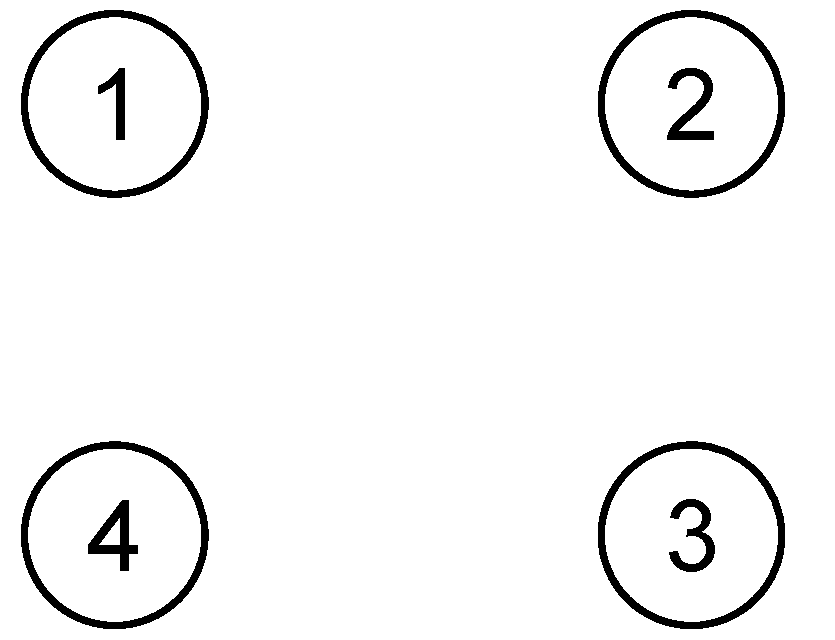
\includegraphics[keepaspectratio,width=0.23\textwidth]{figures/hw-graph-1}
}
\subfloat[]{
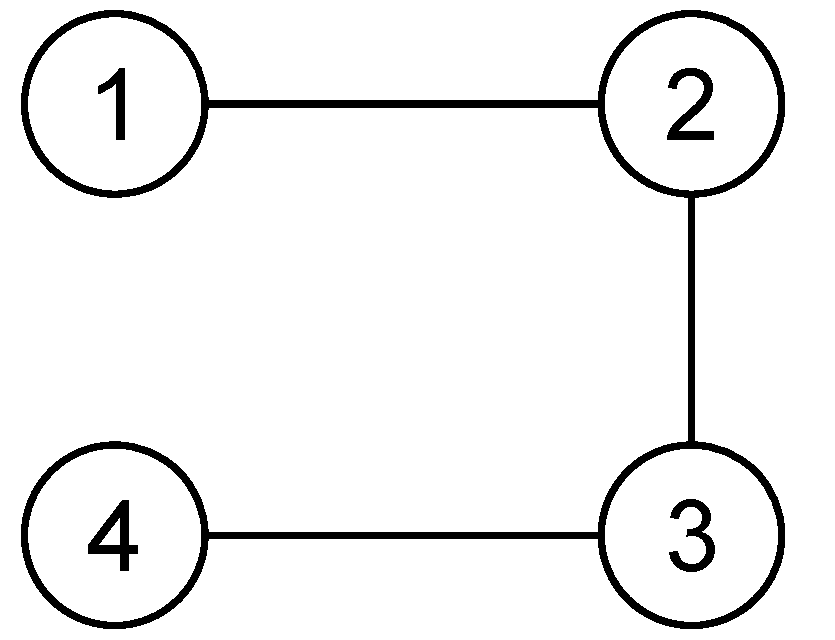
\includegraphics[keepaspectratio,width=0.23\textwidth]{figures/hw-graph-2}
}
\subfloat[]{
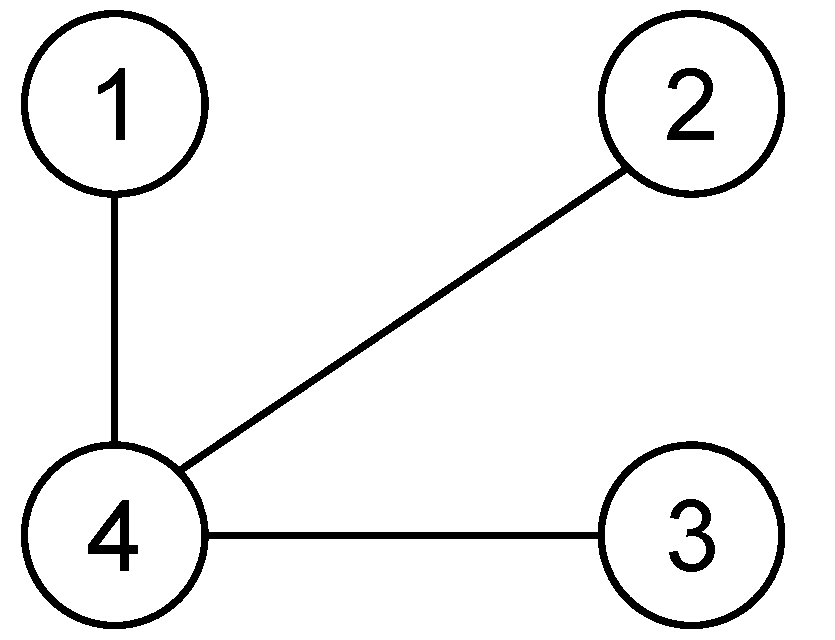
\includegraphics[keepaspectratio,width=0.23\textwidth]{figures/hw-graph-3}
}
\subfloat[]{
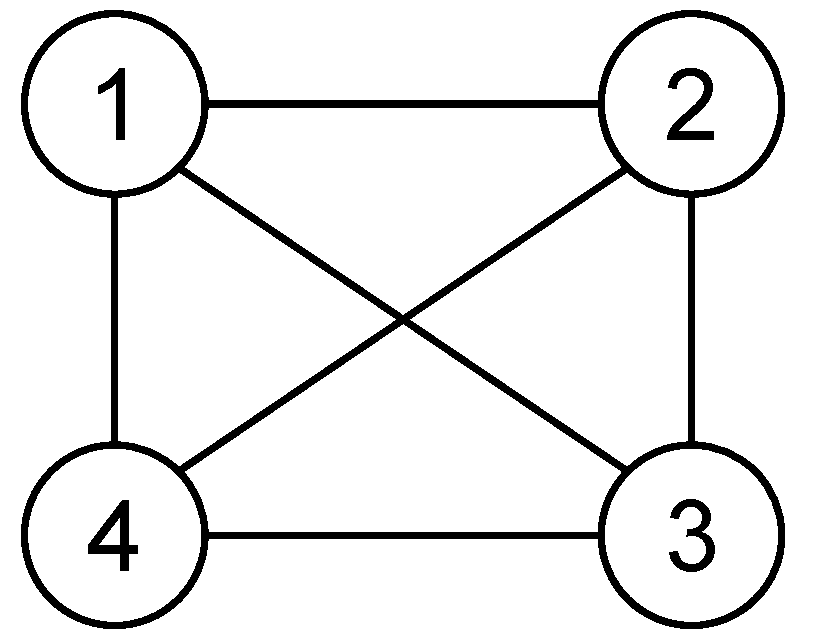
\includegraphics[keepaspectratio,width=0.23\textwidth]{figures/hw-graph-4}
}
\caption{Problem 1(a) graphs. \label{fig:p1a}}
\end{figure}

To judge whether the Laplacian eigenvectors are an \emph{effective} basis for each signal, I use the Laplacian quadratic form:
\[
\mathbf{f}^{\top}L\mathbf{f}=\sum_{(i,j)\in E}(f_i-f_j)^2.
\]
Lower values indicate smoother (lower-frequency) signals, which are represented more efficiently by the low-frequency Laplacian modes.
I use two criteria: (i) smoothness (small \(\mathbf{f}^\top L\mathbf{f}\)) and (ii) compressibility in the Laplacian eigenbasis (how much of the signal sits in a few low-frequency coefficients). Smoothness alone does not guarantee sparse expansion.

\paragraph{Explicit graph matrices (node order \(1,2,3,4\)).}
\[
A_a=\begin{bmatrix}
0&0&0&0\\
0&0&0&0\\
0&0&0&0\\
0&0&0&0
\end{bmatrix},\quad
L_a=D_a-A_a=0.
\]
\[
A_b=\begin{bmatrix}
0&1&0&0\\
1&0&1&0\\
0&1&0&1\\
0&0&1&0
\end{bmatrix},\quad
L_b=\begin{bmatrix}
1&-1&0&0\\
-1&2&-1&0\\
0&-1&2&-1\\
0&0&-1&1
\end{bmatrix}.
\]
\[
A_c=\begin{bmatrix}
0&0&0&1\\
0&0&0&1\\
0&0&0&1\\
1&1&1&0
\end{bmatrix},\quad
L_c=\begin{bmatrix}
1&0&0&-1\\
0&1&0&-1\\
0&0&1&-1\\
-1&-1&-1&3
\end{bmatrix}.
\]
\[
A_d=\begin{bmatrix}
0&1&1&1\\
1&0&1&1\\
1&1&0&1\\
1&1&1&0
\end{bmatrix},\quad
L_d=\begin{bmatrix}
3&-1&-1&-1\\
-1&3&-1&-1\\
-1&-1&3&-1\\
-1&-1&-1&3
\end{bmatrix}.
\]

For the three signals
\[
\mathbf{f}_1=[1,0,0,0],\quad
\mathbf{f}_2=[0,0,0,1],\quad
\mathbf{f}_3=[1,1,0,0],
\]
the smoothness values are:

\begin{table}[htbp]
\centering
\begin{tabular}{lcccc}
\toprule
Signal & Graph (a) & Graph (b) & Graph (c) & Graph (d) \\
\midrule
$\mathbf{f}_1=[1,0,0,0]$ & $0$ & $1$ & $1$ & $3$ \\
$\mathbf{f}_2=[0,0,0,1]$ & $0$ & $1$ & $3$ & $3$ \\
$\mathbf{f}_3=[1,1,0,0]$ & $0$ & $1$ & $2$ & $4$ \\
\bottomrule
\end{tabular}
\caption{Dirichlet energies $\mathbf{f}^{\top}L\mathbf{f}$.}
\end{table}

\noindent\textbf{Short algebra check (representative examples).}
\begin{itemize}[leftmargin=1.2em]
\item Graph (b), \(\mathbf{f}_1=[1,0,0,0]\):
\[
\mathbf{f}_1^\top L_b \mathbf{f}_1
=[1,0,0,0]
\begin{bmatrix}1\\-1\\0\\0\end{bmatrix}
=1.
\]
\item Graph (c), \(\mathbf{f}_2=[0,0,0,1]\): only edges \((1,4),(2,4),(3,4)\) cross values 0 and 1, so
\[
\mathbf{f}_2^\top L_c \mathbf{f}_2=\sum_{(i,j)\in E}(f_i-f_j)^2=1+1+1=3.
\]
\item Graph (d), \(\mathbf{f}_3=[1,1,0,0]\): crossing edges are \((1,3),(1,4),(2,3),(2,4)\), hence
\[
\mathbf{f}_3^\top L_d \mathbf{f}_3=4.
\]
\end{itemize}

\noindent\textbf{Interpretation by graph.}
\begin{itemize}[leftmargin=1.2em]
\item \textbf{Graph (a), no edges:} $L=0$, so all signals have zero energy and all Laplacian eigenvalues are 0. The basis is fully degenerate (no meaningful frequency ordering), so it is not informative.
\item \textbf{Graph (b), path $1$-$2$-$3$-$4$:} all three signals have energy 1 (moderately smooth), but endpoint spikes are not very compressible. For example, for \(\mathbf{f}_1=[1,0,0,0]\), the squared coefficients on the four orthonormal Laplacian eigenvectors are approximately \((0.25,\,0.4268,\,0.25,\,0.0732)\), so all modes are active.
\item \textbf{Graph (c), star centered at node 4:} $\mathbf{f}_1$ is smoothest (energy 1), $\mathbf{f}_3$ is intermediate (2), and $\mathbf{f}_2$ is roughest (3), so effectiveness depends strongly on where the nonzero entries lie relative to the hub.
\item \textbf{Graph (d), complete graph $K_4$:} nonconstant signals are highly nonsmooth (energies 3 or 4), so these binary/local signals are not well aligned with low-frequency structure.
\end{itemize}

\noindent\textbf{Projection details for the path-graph example.}
For \(P_4\), an orthonormal Laplacian eigenbasis is
\[
u_k(j)=\alpha_k\cos\!\left(\frac{(k-1)(j-\tfrac12)\pi}{4}\right),\quad
\alpha_1=\frac12,\ \alpha_{k>1}=\frac{1}{\sqrt2},
\]
with \(j=1,\dots,4\). For \(\mathbf{f}_1=e_1=[1,0,0,0]\), coefficients are \(a_k=u_k^\top e_1=u_k(1)\), so
\[
\begin{aligned}
a_1^2&=\left(\tfrac12\right)^2=\tfrac14,\\
a_2^2&=\left(\tfrac{1}{\sqrt2}\cos\tfrac{\pi}{8}\right)^2=\tfrac12\cos^2\tfrac{\pi}{8}=\tfrac{2+\sqrt2}{8}\approx0.4268,\\
a_3^2&=\left(\tfrac{1}{\sqrt2}\cos\tfrac{\pi}{4}\right)^2=\tfrac14,\\
a_4^2&=\left(\tfrac{1}{\sqrt2}\cos\tfrac{3\pi}{8}\right)^2=\tfrac12\cos^2\tfrac{3\pi}{8}=\tfrac{2-\sqrt2}{8}\approx0.0732.
\end{aligned}
\]
Hence the coefficient energies match the values quoted above.

\subsection*{(b) Computing $f(\mathbf{x})=\mathbf{x}^{\top}L\mathbf{x}$}

\begin{figure}[htbp]
\centering
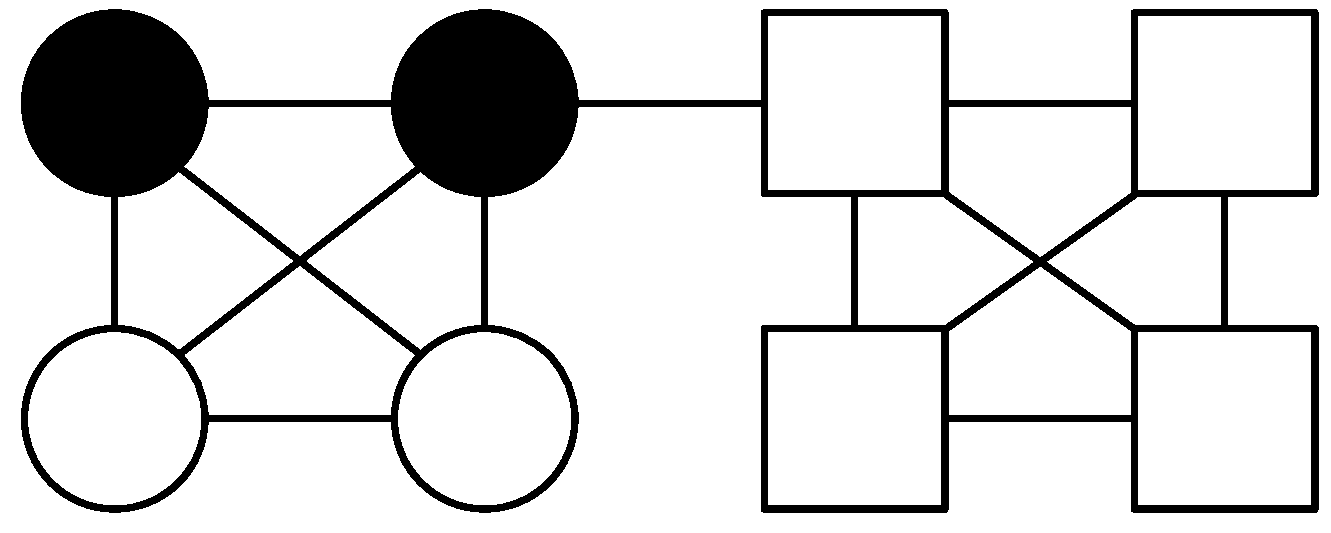
\includegraphics[keepaspectratio,width=0.62\textwidth]{figures/hw-graph-pb}
\caption{Problem 1(b) graph. \label{fig:p1b}}
\end{figure}

Using
\[
\mathbf{x}^{\top}L\mathbf{x}=\sum_{(i,j)\in E}(x_i-x_j)^2,
\]
we evaluate each case:

\paragraph{Constant vector.}
If $\mathbf{x}=c\mathbf{1}$ for any constant $c$, then every edge difference is zero, so
\[
f(\mathbf{x})=\mathbf{x}^{\top}L\mathbf{x}=0.
\]

\paragraph{(i) Ones on squared nodes, zeros on round nodes.}
All edges inside each shape group contribute 0. Only the single bridge edge between the round and square parts crosses from 0 to 1:
\[
f(\mathbf{x})=1.
\]

\paragraph{(ii) Ones on dark nodes, zeros on white nodes.}
In the left 4-node clique, there are 4 dark-white edges. The bridge edge from a dark round node to a white square node adds 1 more. Hence
\[
f(\mathbf{x})=4+1=5.
\]

\paragraph{Intuition.}
$\mathbf{x}^{\top}L\mathbf{x}$ measures edge-wise variation (graph total variation). For binary vectors, it equals the cut size between nodes assigned 1 and nodes assigned 0.

\subsection*{(c) Label Propagation on Figure \ref{fig:p1c}}

\begin{figure}[htbp]
\centering
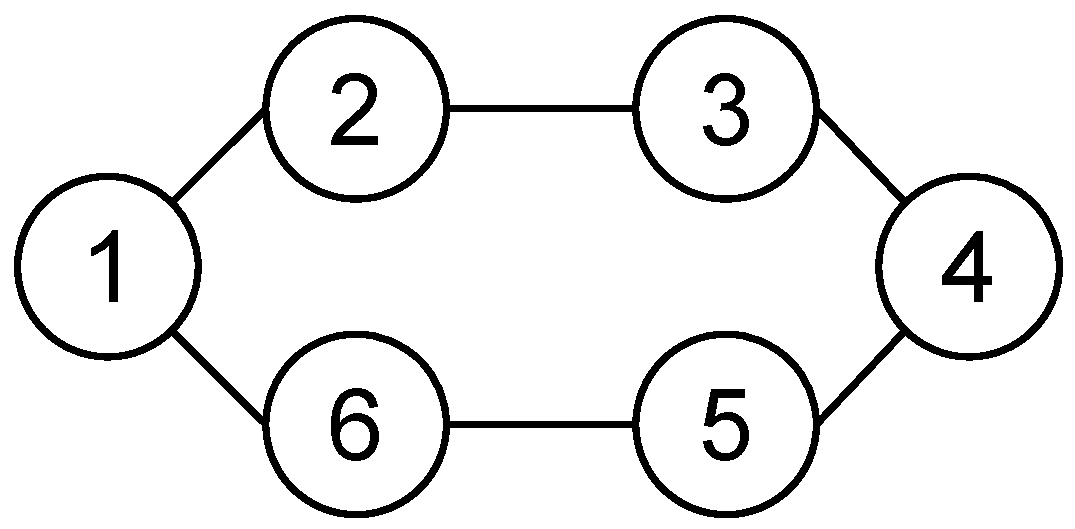
\includegraphics[keepaspectratio,width=0.55\textwidth]{figures/hw-graph-pc}
\caption{Problem 1(c) graph. \label{fig:p1c}}
\end{figure}

I use \textbf{harmonic label propagation} (real-valued labels with clamped seeds). Given labels $y_1=0$ and $y_4=1$, and unlabeled nodes $\{2,3,5,6\}$, each unlabeled node is set to the average of its neighbors:
\[
\begin{aligned}
y_2&=\frac{y_1+y_3}{2}=\frac{y_3}{2},\\
y_3&=\frac{y_2+y_4}{2}=\frac{y_2+1}{2},\\
y_6&=\frac{y_1+y_5}{2}=\frac{y_5}{2},\\
y_5&=\frac{y_6+y_4}{2}=\frac{y_6+1}{2}.
\end{aligned}
\]
Solving gives
\[
y_2=y_6=\frac{1}{3},\qquad y_3=y_5=\frac{2}{3}.
\]
So the final \emph{soft} labeling is
\[
[y_1,y_2,y_3,y_4,y_5,y_6]=\left[0,\frac13,\frac23,1,\frac23,\frac13\right].
\]
Using a 0.5 threshold, the hard labels are
\[
[0,0,1,1,1,0].
\]

\paragraph{Iterations to converge.}
Because the harmonic conditions form a linear system, we can solve it directly (as above), so no iterations are required for the exact answer.

If we instead run synchronous averaging (Jacobi) on the unlabeled nodes, define
\[
\mathbf{x}^{(t)}=[y_2^{(t)},y_3^{(t)},y_5^{(t)},y_6^{(t)}]^\top.
\]
Then
\[
\mathbf{x}^{(t+1)}=P\mathbf{x}^{(t)}+\mathbf{b},
\quad
P=
\begin{bmatrix}
0&\tfrac12&0&0\\
\tfrac12&0&0&0\\
0&0&0&\tfrac12\\
0&0&\tfrac12&0
\end{bmatrix},
\quad
\mathbf{b}=
\begin{bmatrix}
0\\ \tfrac12\\ \tfrac12\\ 0
\end{bmatrix}.
\]
The eigenvalues of \(P\) are \(\{\tfrac12,-\tfrac12,\tfrac12,-\tfrac12\}\), so \(\rho(P)=\tfrac12<1\) and the iteration converges linearly. With \(\mathbf{x}^{(0)}=\mathbf{0}\),
\[
\|\mathbf{x}^{(t)}-\mathbf{x}^\star\|_\infty
\le
\frac{\rho(P)^t}{1-\rho(P)}\|\mathbf{x}^{(1)}-\mathbf{x}^{(0)}\|_\infty
=2^{-t}.
\]
\[
\text{(here }\|\mathbf{x}^{(1)}-\mathbf{x}^{(0)}\|_\infty=\|[0,\tfrac12,\tfrac12,0]^\top\|_\infty=\tfrac12\text{)}
\]
Hence \(t=10\) guarantees error \(\le 10^{-3}\), and \(t=20\) guarantees error \(\le 10^{-6}\).

\subsection*{(d) Confidence-Weighted Laplacian Regularization}

A standard Laplacian-regularized objective is
\[
\min_{\mathbf{f}}\ \|\mathbf{f}-\mathbf{y}\|_2^2+\mu\,\mathbf{f}^{\top}L\mathbf{f}.
\]
To model node-specific confidence in initial labels, replace the uniform fit term with a diagonal confidence matrix $C=\mathrm{diag}(c_1,\ldots,c_n)$:
\[
\min_{\mathbf{f}}\ (\mathbf{f}-\mathbf{y})^{\top}C(\mathbf{f}-\mathbf{y})+\mu\,\mathbf{f}^{\top}L\mathbf{f}.
\]
The solution is
\[
\mathbf{f}^{\star}=(C+\mu L)^{-1}C\mathbf{y}.
\]
Large $c_i$ enforces stronger trust in node $i$'s observed label; small $c_i$ allows more smoothing from neighbors.
In the usual semi-supervised setting, set \(c_i>0\) for labeled nodes and \(c_i=0\) for unlabeled nodes. Then unlabeled entries of \(\mathbf{y}\) can be set arbitrarily (often 0), since they are multiplied by \(c_i=0\).

\paragraph{Toy 2-node illustration.}
For two nodes connected by one edge,
\[
L=\begin{bmatrix}1&-1\\-1&1\end{bmatrix},\quad
C=\begin{bmatrix}c_1&0\\0&c_2\end{bmatrix},\quad
\mathbf{y}=\begin{bmatrix}y_1\\y_2\end{bmatrix}.
\]
Then
\[
C+\mu L=
\begin{bmatrix}
c_1+\mu&-\mu\\
-\mu&c_2+\mu
\end{bmatrix},
\]
and
\[
\mathbf{f}^{\star}
=\frac{1}{(c_1+\mu)(c_2+\mu)-\mu^2}
\begin{bmatrix}
c_2+\mu&\mu\\
\mu&c_1+\mu
\end{bmatrix}
\begin{bmatrix}
c_1 y_1\\
c_2 y_2
\end{bmatrix}.
\]
This explicitly shows how larger \(c_i\) pulls \(f_i^\star\) toward \(y_i\).

In practice, $c_i$ can be determined from:
\begin{itemize}[leftmargin=1.2em]
\item annotator agreement (higher agreement $\Rightarrow$ higher confidence),
\item model-based uncertainty (higher predictive entropy $\Rightarrow$ lower confidence),
\item source reliability or sensor quality metadata,
\item local consistency checks (labels conflicting with trusted neighbors get reduced confidence).
\end{itemize}

\newpage
\section*{Problem 2}

We are given
\[
\min_Y \sum_{(i,j)\in E}\|Y[i]-Y[j]\|_2^2,\qquad Y\in\mathbb{R}^{n\times D}.
\]

\subsection*{(a) Reformulation with the Laplacian}

Let $L=D-A$ be the (unnormalized) graph Laplacian. Then
\[
\sum_{(i,j)\in E}\|Y[i]-Y[j]\|_2^2
=
\operatorname{Tr}(Y^{\top}LY).
\]
So the objective is
\[
\min_Y\ \operatorname{Tr}(Y^{\top}LY).
\]

\subsection*{(b) Computing $Y$ from the Laplacian spectrum}

The unconstrained problem has the trivial collapse solution $Y[i]=\text{constant}$ for all $i$. To obtain a nontrivial embedding, impose standard constraints:
\[
Y^{\top}Y=I_D,\qquad Y^{\top}\mathbf{1}=0.
\]
Using a Lagrangian
\[
\mathcal{L}(Y,\Lambda,\boldsymbol{\nu})
\!=\!
\operatorname{Tr}(Y^\top L Y)
-\operatorname{Tr}\!\big(\Lambda(Y^\top Y-I)\big)
-2\boldsymbol{\nu}^\top Y^\top \mathbf{1},
\]
where \(\Lambda=\Lambda^\top\) (WLOG for orthogonality constraints). Using matrix derivatives for symmetric \(L\):
\[
\nabla_Y\operatorname{Tr}(Y^\top L Y)=2LY,\quad
\nabla_Y\!\left[-\operatorname{Tr}\!\big(\Lambda(Y^\top Y-I)\big)\right]=-2Y\Lambda,\quad
\nabla_Y(-2\boldsymbol{\nu}^\top Y^\top\mathbf{1})=-2\mathbf{1}\boldsymbol{\nu}^\top.
\]
Setting \(\nabla_Y\mathcal{L}=0\) gives
\[
2LY-2Y\Lambda-2\mathbf{1}\boldsymbol{\nu}^\top=0.
\]
Premultiplying by \(\mathbf{1}^\top\), using \(\mathbf{1}^\top L=0\) and \(Y^\top\mathbf{1}=0\), yields \(\boldsymbol{\nu}=0\). Therefore stationarity reduces to the eigen-condition
\[
LY=Y\Lambda,
\]
so each column of \(Y\) is a Laplacian eigenvector. With eigendecomposition $L=U\Lambda U^{\top}$ (eigenvalues $0=\lambda_1\le\lambda_2\le\cdots\le\lambda_n$), Courant-Fischer/Rayleigh-Ritz yields:
\[
Y^{\star}=[u_2,u_3,\ldots,u_{D+1}],
\]
where $u_k$ is the eigenvector for $\lambda_k$.

Hence the embedding coordinates are the first $D$ nontrivial Laplacian eigenvectors (skip the constant eigenvector $u_1$). If the graph is disconnected, skip the full zero-eigenspace and take the next $D$ eigenvectors.
Under these constraints, the minimum objective value is exactly
\[
\operatorname{Tr}\!\big((Y^\star)^\top L Y^\star\big)=\sum_{k=2}^{D+1}\lambda_k
\]
(or, for a graph with multiple zero eigenvalues, the sum of the chosen \(D\) smallest nonzero eigenvalues).

\subsection*{(c) Limitations of this embedding}

\begin{itemize}[leftmargin=1.2em]
\item \textbf{Trivial-collapse risk without constraints:} the raw objective alone is minimized by identical node embeddings.
\item \textbf{Only local smoothness is modeled:} adjacent nodes are forced close, but broader semantic structure may be missed.
\item \textbf{Sensitivity to graph quality:} noisy, missing, or spurious edges directly distort the embedding.
\item \textbf{Disconnected graphs:} multiple zero eigenvalues create ambiguity and can fragment embeddings.
\item \textbf{Scalability:} eigendecomposition is expensive for large graphs.
\item \textbf{No supervision/attributes in the basic form:} node features and labels are ignored unless explicitly added.
\item \textbf{Weak multiscale expressiveness:} a single global quadratic objective may miss hierarchical/community structure across scales.
\end{itemize}

\end{document}
